% ============================================================ %
%  TEMPLATE BODY                                                %
%  Styling lives in preamble.tex, per-document fields live in  %
%  metadata.tex. This file is the actual document content.     %
% ============================================================ %

% ============================================================ %
%  PREAMBLE                                                     %
%  Packages, fonts, spacing, and reusable macros only.          %
%  Per-document content lives in metadata.tex and template.tex. %
% ============================================================ %

% DOCUMENT CLASS SETUP %
\documentclass[12pt, a4paper]{article}

% DOCUMENT PACKAGES %
\usepackage[a4paper, margin=1in]{geometry}
\usepackage{enumitem}
\usepackage{amsmath}
\usepackage{amssymb}
\usepackage{mathtools}
\usepackage{graphicx}
\usepackage{xcolor}
\usepackage{listings}
\usepackage{hyperref}
\usepackage[capitalize, noabbrev]{cleveref}
\usepackage{csquotes}
\usepackage{tocloft}
\usepackage{array}
\usepackage{booktabs}
\usepackage{caption}
\usepackage{subcaption}
\usepackage{mwe}                 % provides \includegraphics{example-image*} placeholders
\usepackage{fancyhdr}
\usepackage{etoolbox}            % powers the optional bibliography toggle

% READABILITY / "AIRY" TYPOGRAPHY SETUP %
\usepackage{setspace}
\setstretch{1.15}
\setlength{\parindent}{0pt}
\setlength{\parskip}{0.6em plus 0.2em}
\usepackage{titlesec}
\titlespacing*{\section}{0pt}{2.4em}{1em}
\titlespacing*{\subsection}{0pt}{1.8em}{0.8em}
\titlespacing*{\subsubsection}{0pt}{1.4em}{0.6em}
\setlist{itemsep=0.4em, topsep=0.6em, parsep=0pt}

% FONT AND ENCODING SETUP %
\usepackage{fontspec}
\usepackage{polyglossia}
\usepackage[Thai]{ucharclasses}
\setdefaultlanguage{english}
\setotherlanguage{thai}
\setTransitionsFor{Thai}{\thaifont}{\normalfont}
\newfontfamily{\thaifont}{THSarabun.ttf}[
    Path=./fonts/,
    BoldFont=THSarabunBold.ttf,
    ItalicFont=THSarabunItalic.ttf,
    BoldItalicFont=THSarabunBoldItalic.ttf,
    Scale=1.23
]
\XeTeXlinebreaklocale "th"
\XeTeXlinebreakskip = 0pt plus 1pt

% Bibliography is a manual thebibliography in main.tex so Tectonic's
% bundled biblatex/biber versions do not have to match.

% CODE BLOCK PACKAGES %
\usepackage{tcolorbox}
\tcbuselibrary{listings, skins, breakable}

% DEFINE GITHUB DARK THEME COLORS %
\definecolor{ghback}{HTML}{0d1117}
\definecolor{ghtext}{HTML}{c9d1d9}
\definecolor{ghborder}{HTML}{30363d}

\lstset{
    basicstyle=\ttfamily\footnotesize\color{ghtext},
    keywordstyle=\color{ghtext}\bfseries,
    commentstyle=\color{ghtext!80},
    stringstyle=\color{ghtext},
    numbers=left,
    numberstyle=\scriptsize\color{white!60!gray},
    numbersep=5pt,
    breaklines=true,
    showstringspaces=false,
    keepspaces=true,
    columns=fullflexible,
    alsoletter={-},
    literate={-}{-}1,
    upquote=true,
    tabsize=4,
}

% CODE BLOCK CONFIGURATION %
\newtcblisting{codeblock}[3][]{
    enhanced,
    breakable,
    colback=ghback,
    colframe=ghborder,
    coltitle=ghtext,
    colupper=ghtext,
    fonttitle=\bfseries\small,
    arc=3mm,
    boxrule=0.5mm,
    left=25pt,
    right=10pt,
    top=5pt,
    bottom=5pt,
    listing engine=listings,
    listing only,
    listing options={
        language=#2,
        basicstyle=\ttfamily\footnotesize\color{ghtext},
        keywordstyle=\color{ghtext}\bfseries,
        numbers=left,
        numberstyle=\scriptsize\color{white!60!gray},
        numbersep=5pt,
        breaklines=true,
        showstringspaces=false,
        keepspaces=true,
        columns=fullflexible,
        alsoletter={-},
        literate={-}{-}1,
        upquote=true,
        tabsize=4,
    },
    title={#3},
    #1
}

% SEMANTIC CALLOUT BOXES %
% Kept to a small, muted set on purpose: Note, Definition, Example, Takeaway.
% Each takes an optional argument to override the default title text, e.g.
%   \begin{notebox}[Note: edge case] ... \end{notebox}
\newtcolorbox{notebox}[1][Note]{
    enhanced, breakable,
    colback=blue!4, colframe=blue!45!black,
    colbacktitle=blue!45!black, coltitle=white,
    fonttitle=\bfseries, title=#1,
    arc=1.5mm, boxrule=0.4mm,
    left=8pt, right=8pt, top=5pt, bottom=5pt,
}
\newtcolorbox{defbox}[1][Definition]{
    enhanced, breakable,
    colback=black!3, colframe=black!55,
    colbacktitle=black!55, coltitle=white,
    fonttitle=\bfseries, title=#1,
    arc=1.5mm, boxrule=0.4mm,
    left=8pt, right=8pt, top=5pt, bottom=5pt,
}
\newtcolorbox{examplebox}[1][Example]{
    enhanced, breakable,
    colback=green!4, colframe=green!30!black,
    colbacktitle=green!30!black, coltitle=white,
    fonttitle=\bfseries, title=#1,
    arc=1.5mm, boxrule=0.4mm,
    left=8pt, right=8pt, top=5pt, bottom=5pt,
}
\newtcolorbox{takeawaybox}[1][Key Takeaway]{
    enhanced, breakable,
    colback=orange!5, colframe=orange!55!black,
    colbacktitle=orange!55!black, coltitle=white,
    fonttitle=\bfseries, title=#1,
    arc=1.5mm, boxrule=0.4mm,
    left=8pt, right=8pt, top=5pt, bottom=5pt,
}

% DISABLE PAGE NUMBER IN TABLE OF CONTENTS %
\tocloftpagestyle{empty}

% RUNNING HEADER / FOOTER (body pages only; cover and TOC stay empty) %
% Left = course code, center = current section, right = author.
\pagestyle{fancy}
\setlength{\headheight}{14pt}
\fancyhf{}
\fancyhead[L]{\small\scshape \coursecode \ \coursename}
% \fancyhead[C]{\small\itshape \rightmark}
\fancyhead[R]{\small \docauthor}
\fancyfoot[C]{\small\thepage}
\renewcommand{\headrulewidth}{0.4pt}
\renewcommand{\footrulewidth}{0pt}
\fancypagestyle{plain}{
    \fancyhf{}
    \fancyfoot[C]{\small\thepage}
    \renewcommand{\headrulewidth}{0pt}
}

% ============================================================ %
%  METADATA                                                     %
%  Edit this file per document. Everything here is the         %
%  "content" you change; the styling stays in preamble.tex.    %
% ============================================================ %

% SHOW BIBLIOGRAPHY? %
% Set to false to hide the "References" section at the end of the document.
\newtoggle{showbibliography}
\toggletrue{showbibliography}

% COVER AND HEADER FIELDS %
\newcommand{\doctitle}{2110413 COMPUTER SECURITY}
\newcommand{\docauthor}{Worralop Srichainont}
\newcommand{\docdate}{\today}
\newcommand{\coursecode}{2110413}
\newcommand{\coursename}{COMPUTER SECURITY}
\newcommand{\assignmentname}{Fundamentals of Cryptography}
\newcommand{\institution}{Computer Engineering, Chulalongkorn University}
\newcommand{\assignmentnumber}{4}
\newcommand{\instructor}{Krerk Piromsopa, Ph.D.}
\newcommand{\studentid}{6632200221}
\newcommand{\duedate}{\today}


% PDF METADATA AND LINK STYLING (needs the fields from metadata.tex) %
\definecolor{linkaccent}{HTML}{1a56db}
\hypersetup{
    pdftitle={\doctitle},
    pdfauthor={\docauthor},
    pdfsubject={\coursecode\ -- \coursename},
    colorlinks=true,
    linkcolor=linkaccent,
    citecolor=linkaccent,
    urlcolor=linkaccent,
    bookmarksnumbered=true,
}

\renewcommand{\subsectionmark}[1]{\markright{#1}}

\begin{document}

    \begin{titlepage}
        \centering
        \thispagestyle{empty}
        \vspace*{4em}

        {\scshape Assignment}

        \vspace{3em}
        {\Huge\bfseries \doctitle}
        \vspace{1.5em}

        \noindent\rule{0.6\textwidth}{0.5pt}
        \vspace{1.5em}

        {\large Assignment \assignmentnumber} \\[0.4em]
        {\large \assignmentname}

        \vfill

        {\large \institution}
        \vspace{1em}

        {\large \docauthor}

        \vspace{0.4em}
        {\normalsize Student ID: \studentid}

        \vspace{2em}
        {\normalsize \docdate}
    \end{titlepage}

    \tableofcontents
    \thispagestyle{empty}
    \clearpage

    \pagenumbering{arabic}

    % \section{Setup}

    %     This report answers Activity~IV (Fundamentals of Cryptography). Commands were run on
    %     macOS (Apple M1 Pro) with Homebrew OpenSSL~3.6.4, ImageMagick~7.1.2-31, Python~3.9.6,
    %     and Tectonic~0.17.0. Scripts live in \texttt{HW04-Homework-04/code/}. Raw OpenSSL
    %     output is in \texttt{code/output/speed/}. Generated figures are in \texttt{docs/images/}.

    %     The macOS \texttt{/usr/bin/openssl} binary is LibreSSL~3.3.6 and does not implement
    %     \texttt{openssl list}. Every cryptographic command below uses
    %     \texttt{/opt/homebrew/opt/openssl@3/bin/openssl}.

    \section{Part I: Cryptanalysis}

        \subsection{Ciphertext}

            The given ciphertext is a short English message written in a classical cipher:
            \begin{quote}
                \texttt{PRCSOFQX FP QDR AFOPQ CZSPR LA JFPALOQSKR.}\\
                \texttt{QDFP FP ZK LIU BROJZK MOLTROE.}
            \end{quote}

        \subsection{English Knowledge}
            
            \subsubsection{Letter frequency}

                Spaces and the period were ignored. There are 59 letters and 20 distinct symbols.

                \begin{table}[h]
                    \centering
                    \begin{tabular}{lc}
                        \toprule
                        Letter & Count \\
                        \midrule
                        P & 7 \\
                        R, O, F & 6 \\
                        Q & 5 \\
                        L & 4 \\
                        S, A, Z, K & 3 \\
                        C, D, J & 2 \\
                        X, I, U, B, M, T, E & 1 \\
                        \bottomrule
                    \end{tabular}
                    \caption{Letter frequencies in the assigned ciphertext.}
                    \label{tab:freq}
                \end{table}

                The three most frequent ranks are \textbf{P} (7), then the tie \textbf{R, O, F} (6).
                In English, E, T, A, O, I, N, S, H, R are usually the most common letters, so P is a
                reasonable first guess for E or S.

            \subsubsection{Short English words}

                \begin{itemize}
                    \item Common two-letter words include \texttt{OF}, \texttt{TO}, \texttt{IN}, \texttt{IS},
                    \texttt{IT}, \texttt{AS}, and \texttt{AN}.
                    \item Common three-letter words include \texttt{THE}, \texttt{AND}, \texttt{FOR}, and \texttt{ARE}.
                \end{itemize}

                In the ciphertext, \texttt{FP} appears twice. \texttt{QDFP FP} is a four-letter
                word followed by that same pair, which matches the English pattern \textbf{THIS IS}.
                Then, we take a look on \texttt{QDR} becomes \texttt{TH?}, so it is certain that R$\rightarrow$E.

                \begin{table}[h]
                    \centering
                    \begin{tabular}{|c|c|c|}
                        \toprule
                        Cipher letters & Shift & Plain Letters \\
                        \midrule
                        \texttt{Q} & +3 & \texttt{T} \\
                        \texttt{D} & +4 & \texttt{H} \\
                        \texttt{F} & +3 & \texttt{I} \\
                        \texttt{P} & +3 & \texttt{S} \\
                        \texttt{R} & +13 & \texttt{E} \\
                        \bottomrule
                    \end{tabular}
                    \caption{First guess of substitution letters}
                    \label{tab:first_sub_table}
                \end{table}

        \subsection{Recovering the plaintext}

            \subsubsection{Complete the substitution table}
                We tried to use the substitution table above and got these:

                \begin{table}[h]
                    \centering
                    \begin{tabular}{|l|l|l|}
                        \toprule
                        Encrypted & Result & Guess \\
                        \midrule
                        \texttt{PRCSOFQX} & \texttt{SE???ITY} & \texttt{SECURITY} \\
                        \texttt{AFOPQ} & \texttt{?IRST} & \texttt{FIRST} \\
                        \texttt{CZSPR} & \texttt{C?USE} & \texttt{CAUSE} \\
                        \texttt{LA} & \texttt{OF} & \texttt{OF} \\
                        \texttt{JFPALOQSKR} & \texttt{?ISFORTU?E} & \texttt{MISFORTUNE} \\
                        \texttt{ZK} & \texttt{AN} & \texttt{AN} \\
                        \texttt{LIU} & \texttt{OLD} & \texttt{OLD} \\
                        \texttt{BROJZK} & \texttt{GERMAN} & \texttt{GERMAN} \\
                        \texttt{MOLTROE} & \texttt{PROVERB} & \texttt{PROVERB} \\
                        \bottomrule
                    \end{tabular}
                    \caption{First guess of substitution letters}
                    \label{tab:first_sub_table}
                \end{table}

    \pagebreak

                Therefore, we got the complete substitution table as

                \begin{table}[h]
                    \centering
                    \begin{tabular}{|c|c|c|}
                        \toprule
                        Cipher letters & Shift & Plain Letters \\
                        \midrule
                        \texttt{P} & +3 & \texttt{S} \\
                        \texttt{R} & +13 & \texttt{E} \\
                        \texttt{C} & +0 & \texttt{C} \\
                        \texttt{S} & +2 & \texttt{U} \\
                        \texttt{O} & +3 & \texttt{R} \\
                        \texttt{F} & +3 & \texttt{I} \\
                        \texttt{Q} & +3 & \texttt{T} \\
                        \texttt{X} & +1 & \texttt{Y} \\
                        \texttt{D} & +4 & \texttt{H} \\
                        \texttt{A} & +5 & \texttt{F} \\
                        \texttt{Z} & +1 & \texttt{A} \\
                        \texttt{L} & +3 & \texttt{O} \\
                        \texttt{J} & +3 & \texttt{M} \\
                        \texttt{K} & +3 & \texttt{N} \\
                        \texttt{I} & +3 & \texttt{L} \\
                        \texttt{U} & +9 & \texttt{D} \\
                        \texttt{B} & +5 & \texttt{G} \\
                        \texttt{M} & +3 & \texttt{P} \\
                        \texttt{T} & +2 & \texttt{V} \\
                        \texttt{E} & +23 & \texttt{B} \\
                        \bottomrule
                    \end{tabular}
                    \caption{Complete substitution letters}
                    \label{tab:sub_table}
                \end{table}

            \subsubsection{Result}
                \begin{quote}
                    \texttt{SECURITY IS THE FIRST CAUSE OF MISFORTUNE.}\\
                    \texttt{THIS IS AN OLD GERMAN PROVERB.}
                \end{quote}

            \begin{notebox}[Note]
                I used around 15 minutes to crack this cipher text manually.
            \end{notebox}

    \pagebreak

        \subsection{Caesar brute-force program}

            The program tries all 26 shifts. It gives one point for each common English word,
            then prints the candidates from highest score to lowest.

            \begin{codeblock}[]{Python}{caesar\_bruteforce.py}
                import sys

                WORDS = {"A", "AN", "THE", "IS", "OF", "TO", "IN", "THIS",
                         "SECURITY", "FIRST", "CAUSE", "MISFORTUNE"}
                SAMPLE = "VHFXULWB LV WKH ILUVW FDXVH RI PLVIRUWXQH."


                def decrypt(text, shift):
                    return "".join(
                        chr((ord(c) - ord("A") - shift) % 26 + ord("A"))
                        if c.isalpha() else c
                        for c in text.upper()
                    )


                def score(text):
                    words = "".join(c if c.isalpha() else " " for c in text).split()
                    return sum(word in WORDS for word in words)


                ciphertext = " ".join(sys.argv[1:]) or SAMPLE
                results = []

                for shift in range(26):
                    plaintext = decrypt(ciphertext, shift)
                    results.append((score(plaintext), shift, plaintext))

                for points, shift, plaintext in sorted(
                        results, key=lambda row: (-row[0], row[1])):
                    print(f"shift={shift:2} score={points}: {plaintext}")
            \end{codeblock}

            For the sample, the first result is:

            \begin{codeblock}[]{text}{Output}
                shift= 3 score=7: SECURITY IS THE FIRST CAUSE OF MISFORTUNE.
            \end{codeblock}

            The homework ciphertext does not fully decrypt with this program because it uses
            different shifts for different letters, rather than one Caesar shift.

    \pagebreak

    \section{Part II: Kasiski examination}

        Vigen\`ere repeats a keyword, so each keyword position acts like a different Caesar
        cipher. Kasiski examination uses repeated ciphertext patterns to estimate the keyword
        length:

        \begin{enumerate}
            \item Find ciphertext strings of at least three letters that appear more than once.
            \item Measure the distance between each pair of repeats.
            \item Find a common factor of the distances. It is a likely keyword length.
            \item Split the text by keyword position and use frequency analysis on each group.
        \end{enumerate}

        After finding the length, the Vigen\`ere cipher becomes several smaller Caesar ciphers,
        which can be cracked separately.

    \pagebreak

    \section{Part III: Block-cipher modes on a bitmap}

        \subsection{Procedure}

            First, I resized the source image and converted it to a 1-bit binary PBM:

            \begin{codeblock}[]{bash}{Image conversion}
                magick docs/images/source.jpg \
                    -resize 2000x2000! -colorspace Gray -threshold 50% \
                    pbm:org.pbm
            \end{codeblock}

            I removed the two-line PBM header and encrypted only the 500{,}000-byte pixel body.
            This size is divisible by AES's 16-byte block size.

            \begin{codeblock}[]{bash}{Encrypt the PBM body}
                openssl enc -aes-256-ecb -in org.x -out enc-ecb.x \
                    -nosalt -nopad -K 001122...ccddeeff

                openssl enc -aes-256-cbc -in org.x -out enc-cbc.x \
                    -nosalt -nopad -K 001122...ccddeeff \
                    -iv 0102030405060708090a0b0c0d0e0f10
            \end{codeblock}

            Finally, I added the original PBM header back to each encrypted body.

        \subsection{Result and analysis}

            \begin{figure}[h]
                \centering
                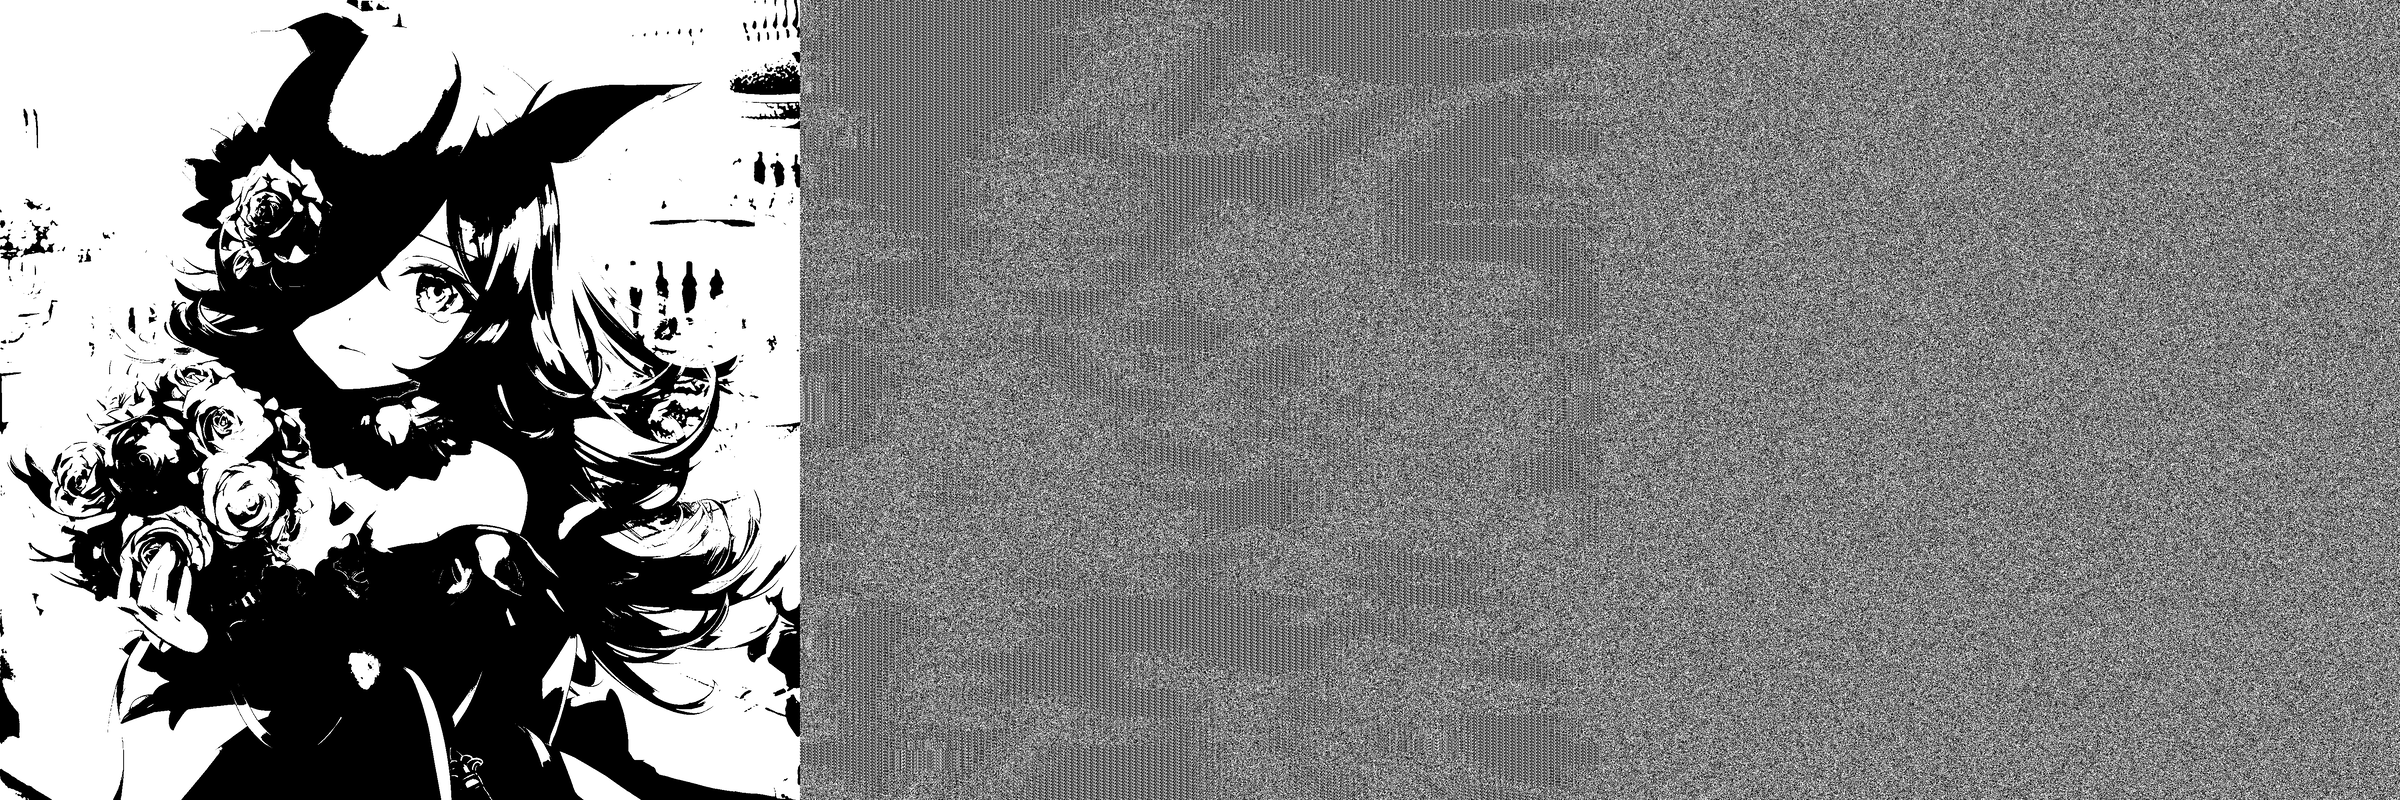
\includegraphics[width=\textwidth]{images/mode-comparison.png}
                \caption{Original 1-bit image (left), AES-256-ECB (middle), AES-256-CBC (right).}
                \label{fig:modes}
            \end{figure}

            ECB encrypts equal plaintext blocks into equal ciphertext blocks, so the picture's
            shape is still visible. CBC mixes each block with the previous encrypted block and
            an IV, so its result looks random. This shows why ECB should not be used for data
            with repeated patterns.

    \pagebreak

    \section{Part IV: Hashing, ciphers, and digital signatures}

        \subsection{Experimental design}

            I used OpenSSL 3.6.4 on an Apple M1 Pro. Each test ran for 3 seconds and was
            repeated three times. The tables show the median result. RC4 and Blowfish need
            OpenSSL's legacy provider.

            \begin{codeblock}[]{bash}{Commands used for Part 4(a)}
                openssl speed -seconds 3 sha1
                openssl speed -seconds 3 -provider legacy -provider default rc4
                openssl speed -seconds 3 -provider legacy -provider default blowfish
                openssl speed -seconds 3 dsa
            \end{codeblock}

        \subsection{Measured results}

            \begin{table}[h]
                \centering
                \small
                \begin{tabular}{lrrrrrr}
                    \toprule
                    Algorithm & 16\,B & 64\,B & 256\,B & 1024\,B & 8192\,B & 16384\,B \\
                    \midrule
                    SHA-1     & 111625 & 391697 & 1092786 & 1830493 & 2316151 & 2333136 \\
                    RC4       & 875828 & 1140693 & 1233343 & 1244972 & 1261681 & 1259033 \\
                    Blowfish  & 121621 & 124320 & 125773 & 125994 & 126441 & 125495 \\
                    \bottomrule
                \end{tabular}
                \caption{Median throughput in 1000s of bytes per second (OpenSSL units).}
                \label{tab:speed-sym}
            \end{table}

            \begin{table}[h]
                \centering
                \begin{tabular}{lrrrr}
                    \toprule
                    DSA size & sign (s) & verify (s) & sign/s & verify/s \\
                    \midrule
                    1024 bit & 0.000068 & 0.000053 & 14708 & 18846 \\
                    2048 bit & 0.000193 & 0.000173 & 5172 & 5770 \\
                    \bottomrule
                \end{tabular}
                \caption{Median DSA sign and verify rates.}
                \label{tab:speed-dsa}
            \end{table}

        \subsection{Performance versus security}

            \begin{itemize}
                \item \textbf{SHA-1} is a fast hash, but collision attacks make it unsafe for
                    new security systems. SHA-256 is a safer choice.
                \item \textbf{RC4} is fast, but its keystream has known biases, so it is obsolete.
                \item \textbf{Blowfish} is slower and has a small 64-bit block size. AES is
                    preferred today.
                \item \textbf{DSA} is much slower because it uses public-key mathematics. It
                    provides signatures, not bulk encryption.
            \end{itemize}

        \subsection{Digital signatures}

            \begin{enumerate}
                \item The sender hashes the message.
                \item The sender signs the hash with their private key.
                \item The receiver hashes the message and checks the signature with the
                    sender's public key.
            \end{enumerate}

            Hashing is fast and detects changes. Public-key signing is slower but proves who
            signed the message. Together they provide integrity, authentication, and
            non-repudiation without applying slow public-key operations to the whole message.

\end{document}
